\section*{Sonstiges}


\Title{Nützliche Formeln}

$$ax^2 + bx + c = 0 \Rightarrow x = \frac{-b \pm \sqrt{b^2 - 4ac}}{2a}$$
$$\binom{n}{k} = \frac{n!}{(n-k)!k!}$$


%------------
% \columnbreak
%------------



\Title{Exponentialfunktion / Logarithmus}

Für die Exponentialfunktion gilt:
\begin{enumerate}[label = (\arabic*)]
	\item $\exp(x) \exp(y) = \exp(x+y)$
	\item $\exp(x) > 1, \quad \forall x > 0$
	\item $x^a = \exp(a \cdot \ln(x))$ und $x^0 = 1$
	\item $\exp(iz) = \cos(z) + i \cdot \sin(z)$
	\item $\exp(i \cdot \frac{\pi}{2}) = i$, $\exp(i \pi) = -1$ und $\exp(2 i \pi) = 1$
\end{enumerate}

Der natürliche Logarithmus $\ln : \, ]0, \infty[ \to \R$ bildet die Umkehrfunktion zu $\exp$ und ist
streng monoton wachsend und stetig. Für den natürliche Logarithmus gilt:

\begin{enumerate}[label = (\arabic*)]
	\item $\ln(1) = 0$
	\item $\ln(e) = 1$
	\item $\ln(a \cdot b) = \ln(a) + \ln(b)$
	\item $\ln(a / b) = \ln(a) - \ln(b)$
	\item $\ln(x^a) = a \cdot \ln(x)$
	\item $x^a \cdot x^b = x^{a + b}$
	\item $(x^a)^b = x^{a \cdot b}$
\end{enumerate}

Im Allgemeinen gilt $\log_b(a) = \frac{\ln(a)}{\ln(b)}$.


\Title{Ableitungs und Integrations Regeln}

\renewcommand\arraystretch{1.8}
\begin{center}
    \begin{tabular}{l|l}
        $F(x)$ & $F'(x) = f(x)$ \\
        \hline
        
        \textbf{Summenregel} & $(f(x) + g(x))' = f'(x) + g'(x)$ \\
		\textbf{Produktregel} & $(f(x) \cdot g(x))' = f'(x) \cdot g(x) + f(x) \cdot g'(x)$ \\
		\textbf{Quotientenregel} & $\left( \frac{f(x)}{g(x)} \right)' = \frac{f'(x) \cdot g(x) - f(x) \cdot g'(x)}{g^2(x)}$ wenn $g(x) \neq 0$ \\
		\textbf{Kettenregel} & $(f(g(x)))' = f'(g(x)) \cdot g'(x)$ \\
		\textbf{Part. Integration} & $\int f'(x) \cdot g(x) dx = f(x) \cdot g(x) - \int f(x) \cdot g'(x) dx$ \\
		\textbf{Substitution} & $\int_{\varphi(a)}^{\varphi(b)} f(x) \; dx = \int_a^b f(\varphi(t)) \cdot \varphi'(t) \; dt$ \\
		\textbf{Logarithmus} & $\int \frac{f'(t)}{f(t)} \; dt = \log(\abs{f(x)})$ \\
    \end{tabular}
\end{center}
\renewcommand{\arraystretch}{1}
  
\Bsp Substitution: Wir wollen $\int \cos(x^2) 2x \; dx$ berechnen dabei gehen wir wie folgt vor:

\begin{enumerate}
	\item Zuerst bestimmen wir die Substitution: $u = x^2$
	\item Nun berechnen wir die Umkehrfunktion: $x = \sqrt{u}$
	\item Dann brauchen wir noch: $\frac{du}{dx} = \frac{dx^2}{dx} = \frac{2x}{1} = 2x \implies dx = \frac{du}{2x}$
	\item Zuletzt können wir dies im Integral einsetzen und erhalten:
		$$\int \cos(x^2) 2x \; dx = \int \cos(u) 2x \; \frac{du}{2x} = \int \cos(u) \; du = \sin(u)$$
	
\end{enumerate}


\Title{Typische Ableitungen und Stammfunktionen}

\renewcommand\arraystretch{1.6}
\begin{center}
    \begin{tabular}{c|c}
        $F(x)$ & $F'(x) = f(x)$ \\
        \hline
            
        $ c $ & $ 0 $ \\
	    $ x^a $ & $ a \cdot x^{a - 1} $ \\
        $ \frac{1}{a+1} x^{a+1} $ & $ x^a $ \\
        $ \frac{1}{a\cdot(n+1)} (ax+b)^{n+1} $ & $ (ax+b)^n $ \\
	    $ \frac{x^{\alpha+1}}{\alpha + 1} $ & $ x^\alpha, \alpha \neq -1 $ \\
        $ \sqrt x $ & $ \frac{1}{2 \sqrt x} $ \\
        $ \sqrt[n] x $ & $ \frac{1}{n} {x}^{ \frac{1}{n} -1 } $ \\
        $ \frac{2}{3} x^{ \frac{3}{2} } $ & $ \sqrt x $ \\
        $ \frac{n}{n+1} x^{ \frac{1}{n}+1 } $ & $ \sqrt[n] x $ \\
	    $ e^x $ & $ e^x $ \\
	    $ \ln(|x|) $ & $ \frac{1}{x} $ \\
        $ \log_a |x| $  &  $ \frac{1}{x \ln a} = \log_a(e) \frac{1}{x} $ \\
        $ a^{cx} $ & $ a^{cx} \cdot c \ln a $ \\
        $ x^x $ & $ x^x \cdot (1+\ln x) \quad \scriptstyle x > 0 $ \\
        $ x \cdot (\ln |x| - 1) $  &  $ \ln |x| $ \\
    \end{tabular}
\end{center}
\renewcommand{\arraystretch}{1}


\Title{Funktionen}

\begin{center}
	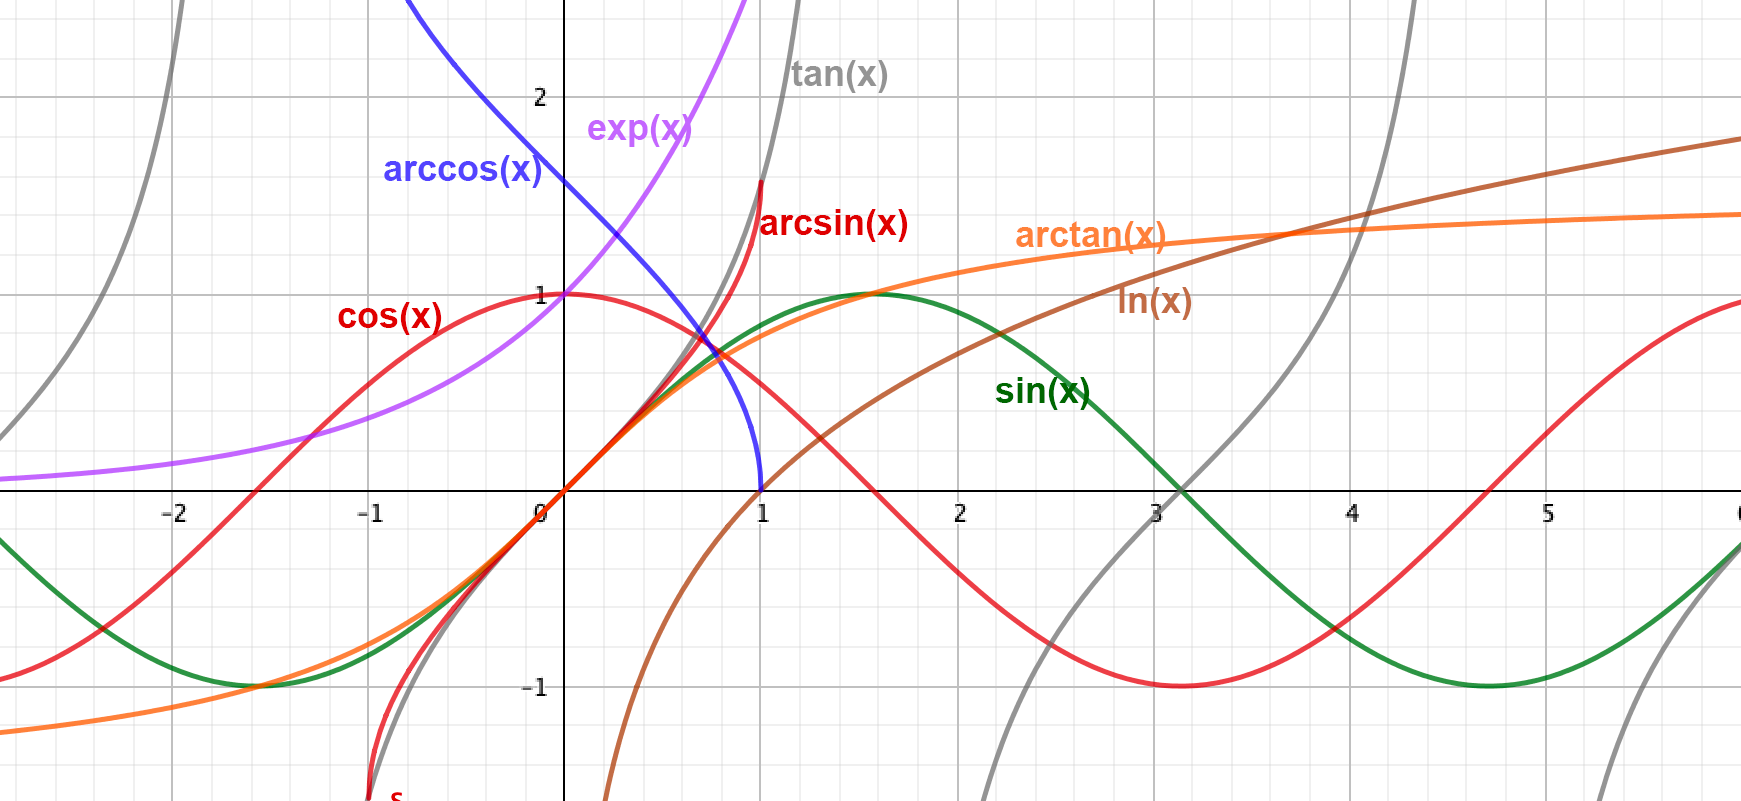
\includegraphics[width=\linewidth]{assets/funktionen.png}
\end{center}
